\documentclass[t,handout,professionalfont,serif]{beamer}
\usetheme{Madrid}
\usepackage[T1]{fontenc}
\usepackage[english]{babel}
\usepackage{graphicx}
\usepackage{setspace}
\usepackage{amsfonts,amssymb}
\usepackage{tikz}
\usepackage{MnSymbol}
\usepackage{tabularx}
\usepackage{amsmath}
\usepackage{url}
\usepackage{interval}
\usepackage{booktabs}
\usetikzlibrary{shapes.geometric, arrows,automata,positioning}
%\usepackage{scrextend}
\usepackage{mathtools}
\usepackage{minted}
%\usepackage{scalerel}
%\usepackage{lipsum}\label{key}
%\usepackage{centernot}
%\usefonttheme[onlymath]{serif}
%\usepackage{pxfonts}
%\setbeamersize{text margin left=3mm,text margin right=3mm} 
\setbeamerfont{caption}{size=\tiny}

\makeatother
\setbeamertemplate{footline}
{
	\leavevmode%
	\hbox{%
		\begin{beamercolorbox}[wd=.2\paperwidth,ht=2.25ex,dp=1ex,center]{author in head/foot}%
			\usebeamerfont{author in head/foot}\insertshortauthor
		\end{beamercolorbox}%
		\begin{beamercolorbox}[wd=.8\paperwidth,ht=2.25ex,dp=1ex,center]{title in head/foot}%
			\usebeamerfont{title in head/foot}\insertshortinstitute\hspace*{3em}
			%\insertframenumber{} / \inserttotalframenumber\hspace*{1ex}
	\end{beamercolorbox}}%
	\vskip0pt%
}
\makeatletter
\setbeamertemplate{navigation symbols}{}

\AtBeginSection[]{
	\begin{frame}
		\vfill
		\centering
		\begin{beamercolorbox}[sep=8pt,center,shadow=true,rounded=true]{title}
			\usebeamerfont{title}\insertsectionhead\par%
		\end{beamercolorbox}
		\vfill
	\end{frame}
}


\title[New Monte Carlo Algorithms for Multi-Dimensional Integration with Hardware Acceleration]{New Monte Carlo Algorithms for Multi-Dimensional Integration with Hardware Acceleration}
\author{Andrea Pasquale}
\institute[Università degli Studi di Milano - Corso di Laurea Magistrale in Fisica ]{Università degli Studi di Milano - Corso di Laurea Magistrale in Fisica }
\date{13th July 2021}
\begin{document}
	\begin{frame}
		\maketitle
	\end{frame}

\section{Monte Carlo integration in HEP}

\begin{frame}{Monte Carlo Integration}
	\scriptsize
Monte Carlo (MC) integration enables us to to solve complex multi-dimensional integrals
\begin{equation}
	I = \int_{V}   f(\textbf{x}) d \textbf{x} \ 
\end{equation}
by simply sampling the function $f$ in $N$ random points:
\begin{equation}
	I \approx I_{\text{MC}} = V \frac{1}{N} \sum_{\textbf{x}_i \in V} f(\textbf{x}_i) = V \langle f \rangle \ 
\end{equation}
The variance of $I_\text{MC}$  can be computed using the previously sampled points as
\begin{equation}
	\sigma^2_I \approx \sigma^2_\text{MC}  = \frac{1}{N-1} \Big[ 
	V^2 \langle  f^2 \rangle 
	- I^2_{\text{MC}}\Big] \Rightarrow \sigma_\text{MC} \sim \frac{1}{\sqrt{N}}
\end{equation}

\textbf{Advantage of MC}: the error depends only on $N$ $\nRightarrow$ quadrature integration
\vspace{0.3cm}

\textbf{Aim of MC algorithms}: reduce the variance in the integral estimate through
\begin{itemize}
	\item stratified sampling techniques $\Rightarrow$ divide the integration region
	\item importance sampling techniques $\Rightarrow$ sample using non-uniform distribution
\end{itemize}


	
	
\end{frame}






\begin{frame}{Monte Carlo integration in HEP}
	\scriptsize
	\tikzstyle{first} = [rectangle, rounded corners, minimum width=3cm, minimum height=1cm,text centered, draw=black, fill=red!30]
	\tikzstyle{second} = [rectangle, rounded corners, minimum width=3cm, minimum height=1cm, text centered, draw=black, fill=green!30]
	\tikzstyle{software} = [rectangle, rounded corners, minimum width=3cm, minimum height=1cm, text centered, draw=black, fill=blue!30]
	\tikzstyle{arrow} = [thick,->,>=stealth]
	\tikzstyle{arrow1} = [thick,->,>=stealth, dashed]
	\tikzstyle{arrow2} = [thick,-,>=stealth]
	What does Monte Carlo integration have to deal with High Energy Physics?
	
\begin{figure}
		
		\centering
		\begin{tikzpicture}[node distance=2cm]
			
			\setstretch{1}
			{
				
				\node (experiment) [first] {LHC at CERN};
				\node(data)[first,below of = experiment] {Experimental Data};
				\node(theory)[first, right of = experiment, xshift = +5cm]{Standard Model};
				\node(predictions)[first, below of = theory] {Theoretical predictions};
				\node(integration)[first, below of = predictions, yshift = -0.5cm, align = center] {Monte Carlo \\ Integration Techniques};
				\node(apparatus)[first, below of = data, yshift = -0.5cm] {Technlogical development};
				\node(question)[first, right of = data, xshift = + 1.5cm,align = center] {Can the SM explain\\ the data?};
				%\node (importance) [method, below of = vegas, right of = vegas, align = center] {importance\\sampling};
				%\node (stratified) [method, below of = vegas, left of = vegas, align = center] {stratified\\sampling};
				%\node(vegasflow)[software, right of = importance, xshift = +2cm] {\texttt{VegasFlow}};
				%\node (adaptive) [method, below of = stratified,align=center] {adaptive\\stratified\\sampling};
				%\node(vegas+)[algorithm, below of = importance] {\texttt{VEGAS+}};
				%\node(vegasflowplus)[software, right of = vegas+, xshift = +2cm] {\texttt{VegasFlowPlus}};
			}
			
			\draw [arrow] (experiment) -- (data);
			\draw [arrow] (theory) -- (predictions);
			\draw[arrow](data) -- (question);
			\draw[arrow]  (predictions) -- (question);
			\draw[arrow]  (apparatus) --  (data);
			\draw[arrow]  (integration) -- (predictions);
			

		\end{tikzpicture}
		\label{scheme}
	\end{figure}
		
\end{frame}

\begin{frame}{The Standard Model}
	\scriptsize
	In the Standard Model we can predict the value of an observable as a series of terms
	\begin{equation}
		d\sigma = d\sigma^{\text{LO}} + d\sigma^{\text{NLO}} + d\sigma^{\text{NNLO}} \dots  \ .
	\end{equation}
every term is computed as
\begin{equation}
	d\sigma \sim \underbrace{|\mathcal{M}(p_1,\dots, p_n)|^2}_{\substack{\text{scattering} \\ \text{amplitude}}} \times \underbrace{d\Phi_n(p_1,\dots, p_n)}_{\substack{\text{phase-space}\\ \text{density}}}  
\end{equation}
High-dimensional integrals arise from:
\begin{itemize}
	\item  $d\Phi_n(p_1,\dots, p_n) $  :  $D_\text{integral} = 3 \times n - 4$ 
	\item $\mathcal{M}^{\text{L- loops}}(p_1,\dots, p_n)$ :  $D_\text{integral} = 4 \times l$ 
\end{itemize}
\vspace{0.5cm}

Higher order terms involve more looops and more particles resulting in complicated integrals to evaluate. Futhermore, they are usually peaked in small region of the integration volume near kinematics divergences which are difficult to sample.
\end{frame}




\begin{frame}{Cost of Monte Carlo Integration}
	\scriptsize
	\textbf{Problem}: MC integration is computationally expensive for high accuracy requirements!
\begin{columns}
	\begin{column}{0.5 \textwidth}
		\begin{itemize}
			\item High CPU resources
		\end{itemize}
		\begin{figure}[h]
			\centering
			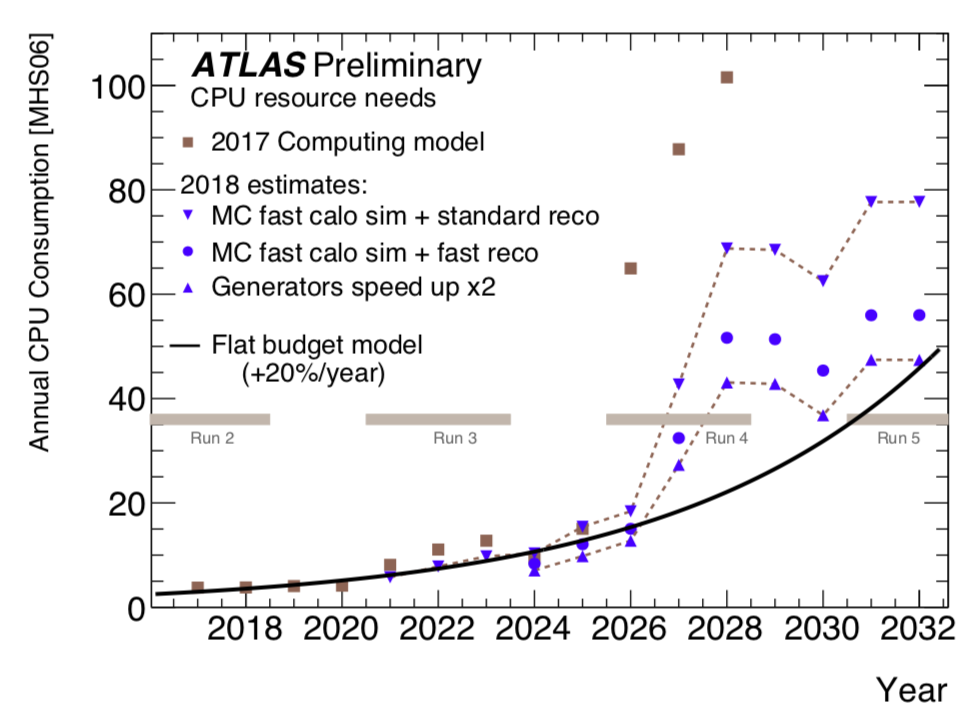
\includegraphics[width = \columnwidth]{../tex/images/CPU-cost.png}
				\label{CPU cost}
			\end{figure}
	\end{column}
	\begin{column}{0.5 \textwidth}
		\begin{itemize}
			\item Long computational times
		\end{itemize}
	\begin{figure}[h]
		\centering
		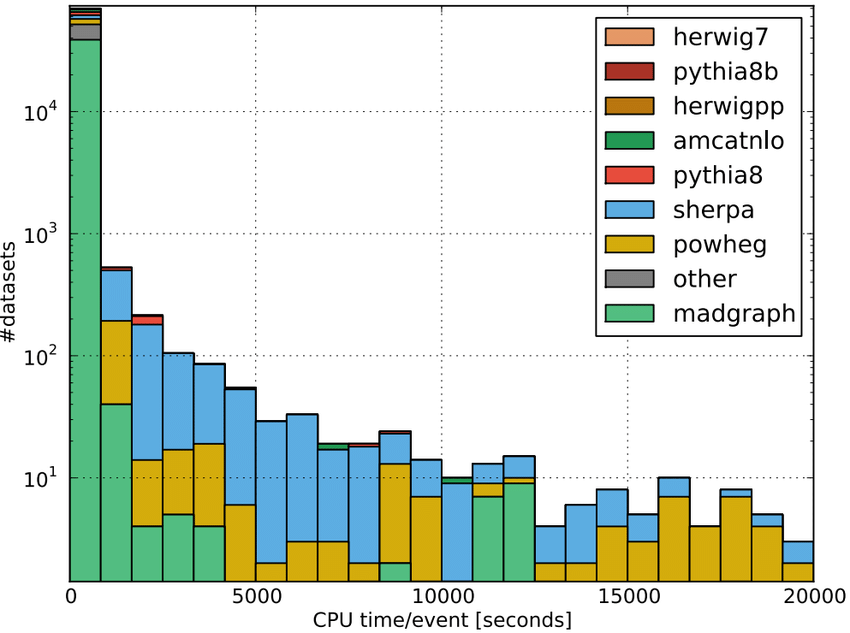
\includegraphics[width = \columnwidth]{../tex/images/CPU-time.png}
		\label{CPU1 cost}
	\end{figure}
\end{column}
\end{columns}
The current integration algorithms  will not be able to produce theoretical predictions that match the precision of the experimental data in the next years.
	\end{frame}

\begin{frame}{Solutions and aim of the thesis}
	\scriptsize
		\textbf{Question}:
		\begin{itemize}
			\item How can we obtain high-accuracy predictions 
			at acceptable CPU costs and computational times?
		\end{itemize}



	
	\vspace{0.5cm}
	\textbf{Solution}:
	\begin{enumerate}
		\item Develop new algorithms for multi-dimensional integration.
		\item Look at new computer architecture: GPUs or multi-threading CPUs. 
	\end{enumerate}
		\vspace{0.5cm}
\textbf{Outline of the thesis}:
\begin{itemize}
	\item Study of  a new MC integrator effective with HEP integrands
	\item Implementation using hardware acceleration to lower the CPU usage
	\item Benchmark the performance of the new algorithm
\end{itemize}
\end{frame}
\section{Algorithms and implementation}

\begin{frame}{Algorithms}
	\scriptsize
	We start from \texttt{VEGAS}, an algorithm for adaptive multi-dimensional MC integration implemented by Lepage in 1977.
			\tikzstyle{algorithm} = [rectangle, rounded corners, minimum width=2cm, minimum height=1cm,text centered, draw=black, fill=red!30]
	\tikzstyle{method} = [rectangle, rounded corners, minimum width=2cm, minimum height=1cm, text centered, draw=black, fill=green!30]
	\tikzstyle{software} = [rectangle, rounded corners, minimum width=2cm, minimum height=1cm, text centered, draw=black, fill=blue!30]
	\tikzstyle{arrow} = [thick,->,>=stealth]
	\tikzstyle{arrow1} = [thick,->,>=stealth, dashed]
	
	\begin{figure}
		
		\centering
		\begin{tikzpicture}[node distance=1.5cm]
			
			\setstretch{1}
			{
				
				\node (vegas) [algorithm] {\texttt{VEGAS}};
				\node (importance) [method, below of = vegas, right of = vegas, align = center, yshift = - 0.75cm] {importance\\sampling};
				\node (stratified) [method, below of = vegas, left of = vegas, align = center] {stratified\\sampling};
				\node(vegasflow)[software, right of = importance, xshift = +2cm] {\texttt{VegasFlow}};
				\node (adaptive) [method, below of = stratified,align=center] {adaptive\\stratified\\sampling};
				\node(vegas+)[algorithm, below of = adaptive, right of = adaptive] {\texttt{VEGAS+}};
				\node(vegasflowplus)[software, right of = vegas+, xshift = +2cm] {\texttt{VegasFlowPlus}};
			}
			
			\draw [arrow] (vegas) -- (importance);
			\draw [arrow] (vegas) -- (stratified);
			\draw[arrow] (importance) -- (vegasflow);
			\draw[arrow] (adaptive) -- (vegas+);
			\draw[arrow] (importance) -- (vegas+);
			\draw[arrow] (vegas+) -- (vegasflowplus);
			\draw[arrow1] (stratified) -- (adaptive);
		\end{tikzpicture}
	\end{figure}
We focus our analysis on \texttt{VEGAS+}, a new algorithm which employs a novel adaptive stratified sampling technique.
	
\end{frame}

\begin{frame}{New features of \texttt{VEGAS+}}
	\scriptsize
	\vspace{-0.5cm}
	{ % begin box to localize effect of arraystretch change
		\renewcommand{\arraystretch}{2.0}
	
		\begin{table}
		\centering
		\begin{tabular}{l| l  } 
		\textbf{Adaptive stratified sampling of \texttt{VEGAS+}} & 	\textbf{Stratified sampling of \texttt{VEGAS}}    \\
			\hline
			\vtop{
				\hbox{Each hypercube $h$ is sampled with a}
				\hbox{different number of points $n_h$  which}
				\hbox{are adjusted iteratively. The integral and}
				\hbox{the variance are now computed as}}  
		
				
				

				& 	\vtop{\hbox{Each hypercube $h$ is sampled with the  }
					\hbox{same number of points $n_\text{ev}$. The integral }
					\hbox{and the  variance are computed as}}
							\\ 
			  $I = \frac{V}{N_\text{st}^D}\sum_h \frac{1}{n_h} \sum_{\textbf{x} \in h} f(\textbf{x})  = \sum_h I_h   $  & $I = \frac{V}{N_\text{st}^D}\sum_h \bigg(\frac{1}{n_\text{ev}} \sum_{\textbf{x} \in h} f(\textbf{x}) \bigg) = \sum_h I_h   $ \\ 
			  $ \sigma^2_I = \sum_h \sigma^2_h  $ & $ \sigma^2_I = \sum_h \sigma^2_h  $ \\ 
		\hline
			
		\end{tabular}
	\end{table}
}
\textbf{Samples redistribution algorithm}
\begin{enumerate}
	\item Choose number of stratifications $N_\text{st} = \lfloor (N_\text{ev}/4)^{1/D}\rfloor $
	\item Accumulate the variance in each hypercube:
	$$ \sigma^2_h \approx \frac{V_h^2}{n_h} \sum_{\textbf{x} \in V_h} f^2(\textbf{x}) - \bigg( \frac{V_h}{n_h} \sum_{\textbf{x} \in V_h} f(\textbf{x})\bigg)^2  $$
	\item Replace the variance with $d_h$ : $d_h \equiv \sigma_h^\beta$ with $\beta \geq 0$
	\item Recalculate the number of samples for each hypercube for the next iteration
	$$ n_h = \text{max} \big(2, d_h / \sum_{h'} d_{h'}\big)  $$
\end{enumerate}
	

\end{frame}

\begin{frame}{Motivation}
	\scriptsize
	\vspace{-0.3cm}
	Why do we choose to implement the \texttt{VEGAS+} algorithm?
	\vspace{-0.5cm}
		\begin{columns}
		\begin{column}{0.6 \textwidth}
			\begin{figure}
				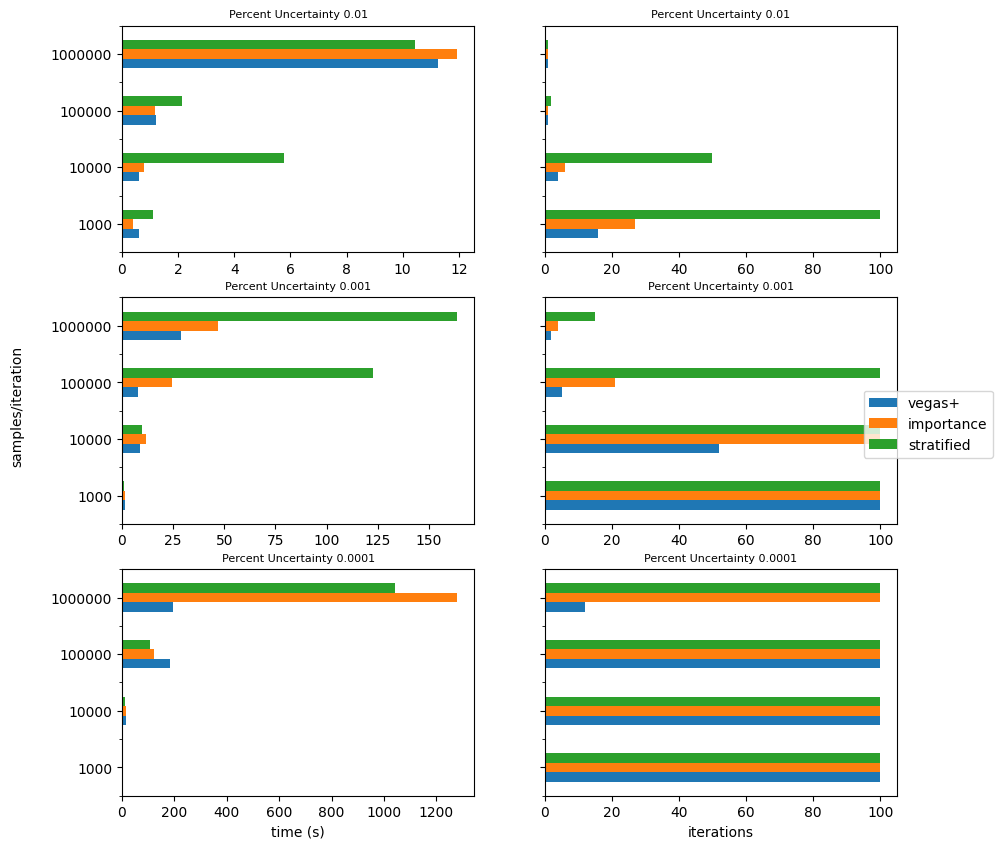
\includegraphics[ height = 6cm]{../tex/images/dy_aa.png}
			\end{figure}
		\tiny
			For the DY LO partonic level cross setion \texttt{VEGAS+} converge within the limit of 100 iterations when aiming at 0.0001\%  percent uncertainty.
		\end{column}


	
		\begin{column}{0.4 \textwidth}
			\tiny
			\begin{figure}[h]
				\centering
				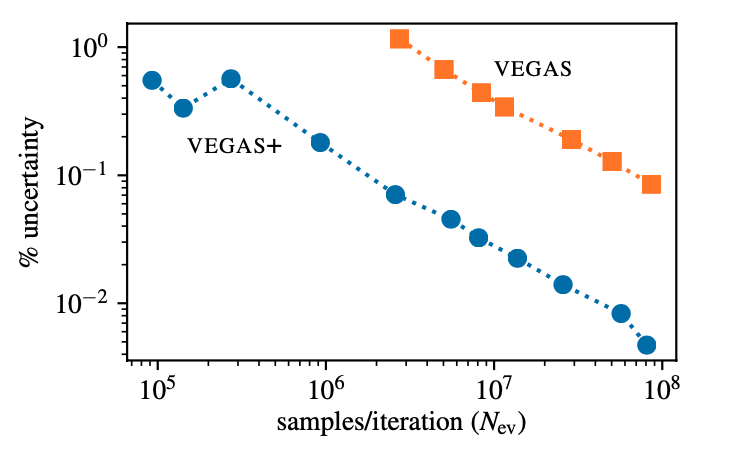
\includegraphics[width=\columnwidth]{../tex/images/VEGAS-VEGAS+.png}
				\label{vegas_vegas+}
			\end{figure}
			\vspace{-0.5cm}
		$$
			\int_0^1 d^8 x \sum_{i=1}^3 e^{-50 |\textbf{x}- \textbf{r}_i|} \ 
		$$
		\vspace{-0.5cm}
		\begin{eqnarray*}
			\textbf{r}_1 &= (0.23,\dots,0.23)  \ ,\\
			\textbf{r}_2 &= (0.39,\dots,0.39)  \ , \\
			\textbf{r}_3 &=(0.74,\dots,0.74)   \ .
		\end{eqnarray*}
			
		\texttt{VEGAS+} can overcome the poor performance of \texttt{VEGAS} with non-separable integrands.
		The redistribution of samples helps the importance sampling algorithm finding the peaks correctly.
			
		\end{column}
		
	\end{columns}
	
\end{frame}



\begin{frame}[fragile]{\texttt{VegasFlow}}
	\scriptsize
\texttt{VegasFlow}: implementation of the Vegas importance sampling using hardware acceleration.

This is possible thanks to the \texttt{TensorFlow} library which enable us to distribute python code to hardware acceleration devices.
		\begin{columns}
		\begin{column}{0.5 \textwidth}
			\tiny
			Better computational times for physical integrand!
			\vspace{-0.3cm}
			\begin{figure}
				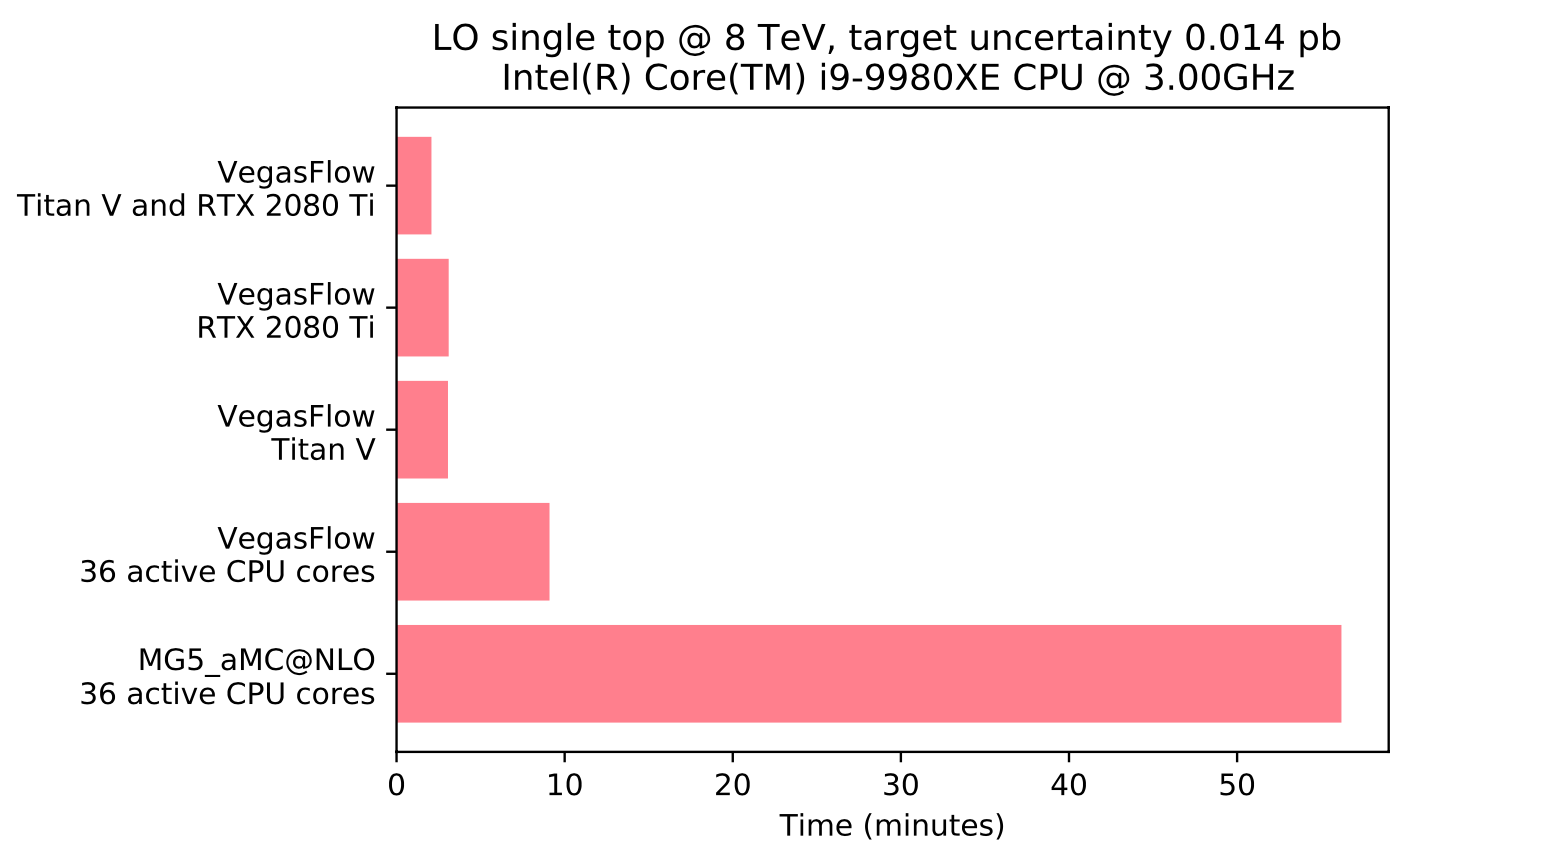
\includegraphics[ width = \columnwidth]{../tex/images/vf_singletop.png}
				
				\vspace{-0.2cm}
					\caption{Comparison of a Leading Order calculation ran in both \texttt{VegasFlow} 
					 and MG5\_aMC@NLO . For the same level 
					of target accuracy \texttt{VegasFlow} is faster than  MG5\_aMC@NLO when using both CPUs and GPUs devices. }

				
				
			\end{figure}
		\end{column}
		\begin{column}{0.5 \textwidth}
			\begin{figure}
				\vspace{-0.6cm}
				\tiny
				Advantage of graph implementation!
				
				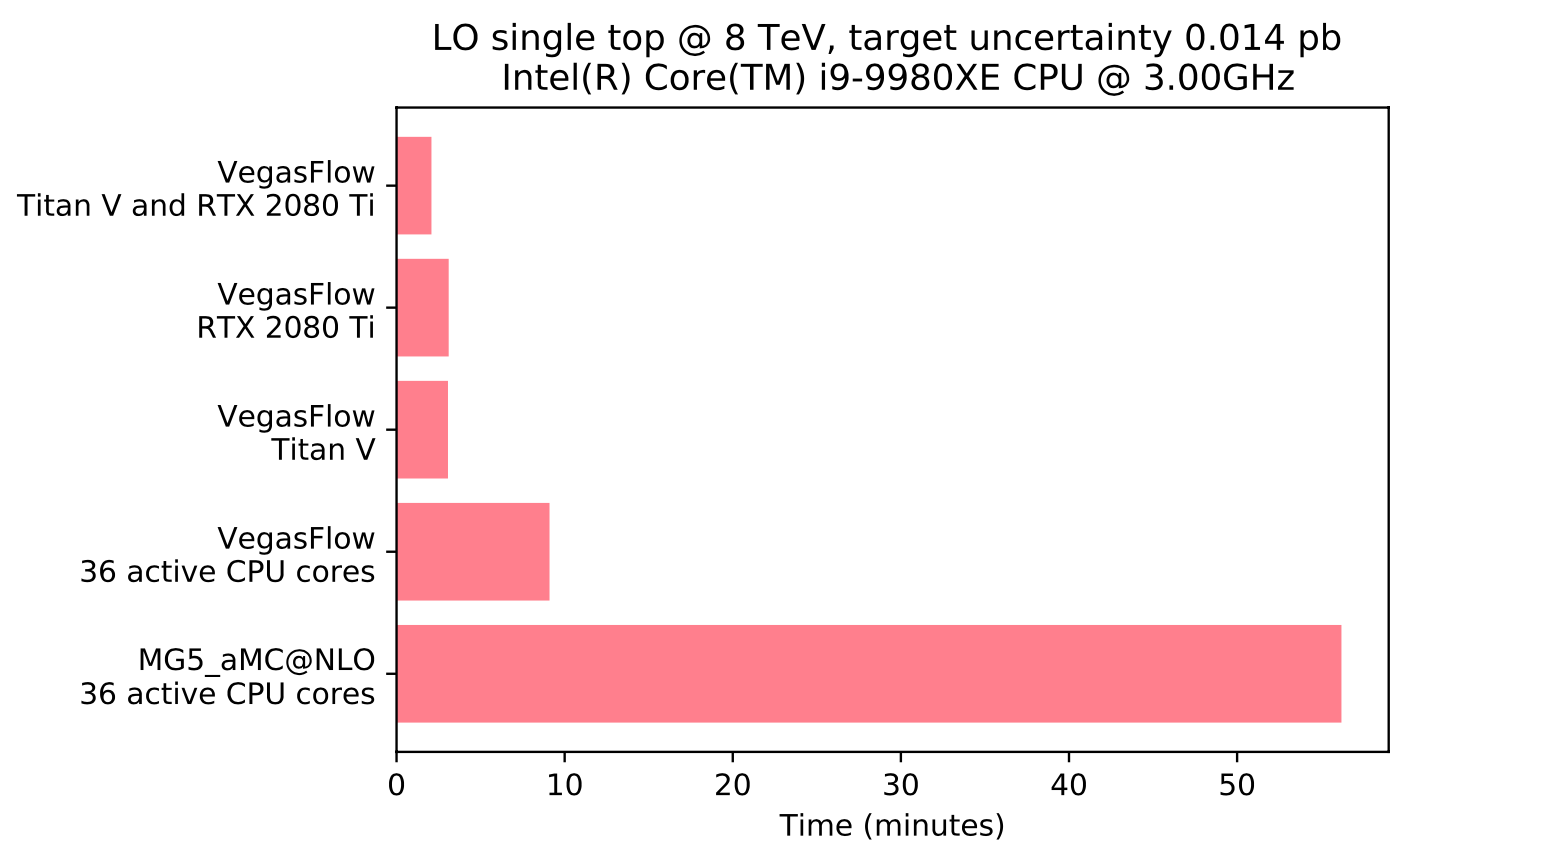
\includegraphics[ width = \columnwidth]{../tex/images/graph_mode.png}
				
								\vspace{-0.3cm}
				\caption{Comparison of performance between the eager and graph compilation TensorFlow mode. The results are shown as a ratio of the time it took the eager computation to complete one iteration.}
			\end{figure}
		\end{column}
		
	\end{columns}

Our aim is to implement the \texttt{VEGAS+} algorithm within the \texttt{VegasFlow} library, empowering the algorithm by enabling to run the integration in GPUs.




	
\end{frame}

\begin{frame}{Implementation of \texttt{VegasFlowPlus}}
	\scriptsize
	\textbf{Details of the implementation}
	\begin{itemize}
		\item Class derived from the \texttt{VegasFlow} integrator (same importance sampling algorithm)
		\item Adding stratified sampling : \texttt{generate\_samples\_in\_hypercubes} + other modifications
		\item New feature of \texttt{VEGAS+}: \texttt{redistribute\_samples}
	\end{itemize}
	
	\vspace{2cm}
	
	\textbf{Problems during the implementation}:
	\begin{itemize}
		\item Number of events not constant $\Rightarrow$ require \texttt{input\_signature}
		\item Memory problem caused by \texttt{tf.repeat} $\Rightarrow$ limit on number of hypercubes
	\end{itemize}
\end{frame}



\section{Benchmark results}

\begin{frame}{Benchmark results}
	\scriptsize
	Integration setup:
	\begin{itemize}
		\item warm-up of 5 iterations with 1M samples with grid refinement ($\alpha=1.5$)
		\item 1M samples for each iteration after the warm-up 
	\end{itemize}
\tiny
	\begin{table}
		\centering
		\begin{tabular}{c| c| c| c | c | c   } 
			Integrator Name & Class & warm-up method& integration method  \\
			\hline
			Importance Sampling & \texttt{VegasFlow} & importance & importance \\ 
			Classic VEGAS & \texttt{VegasFlowPlus}& importance + stratified & importance + stratified \\
			VEGAS/VEGAS+ hybrid  & \texttt{VegasFlowPlus} & importance + adaptive & importance + stratified \\
			VEGAS+ & \texttt{VegasFlowPlus}& importance + adaptive & importance + adaptive \\ 
			\hline
			
		\end{tabular}
		\label{only table}
	\end{table}
\scriptsize

Hardware setup:
\begin{itemize}
	\item professional-grade CPU: Intel(R) Core(TM) i9-9980XE - 36 threads
	\item professional-grade GPU: NVIDIA Titan V
\end{itemize}

\vspace{0.5cm}
We would like to answer the following questions:
\begin{itemize}
	\item Can \texttt{VegasFlowPlus} perform better than \texttt{VegasFlow}?
	\item Can \texttt{VegasFlowPlus} benefit from hardware acceleration?
	\item Can we provide the user with a \emph{recipe} describing which integrators works best depending on the integral to compute?
\end{itemize}	
	
\end{frame}

\begin{frame}{Gaussian Integral Benchmark - Dimension 4}
	\tiny
\vspace{-0.5cm}
\begin{columns}
	\begin{column}{0.6 \textwidth}
		\begin{figure}
			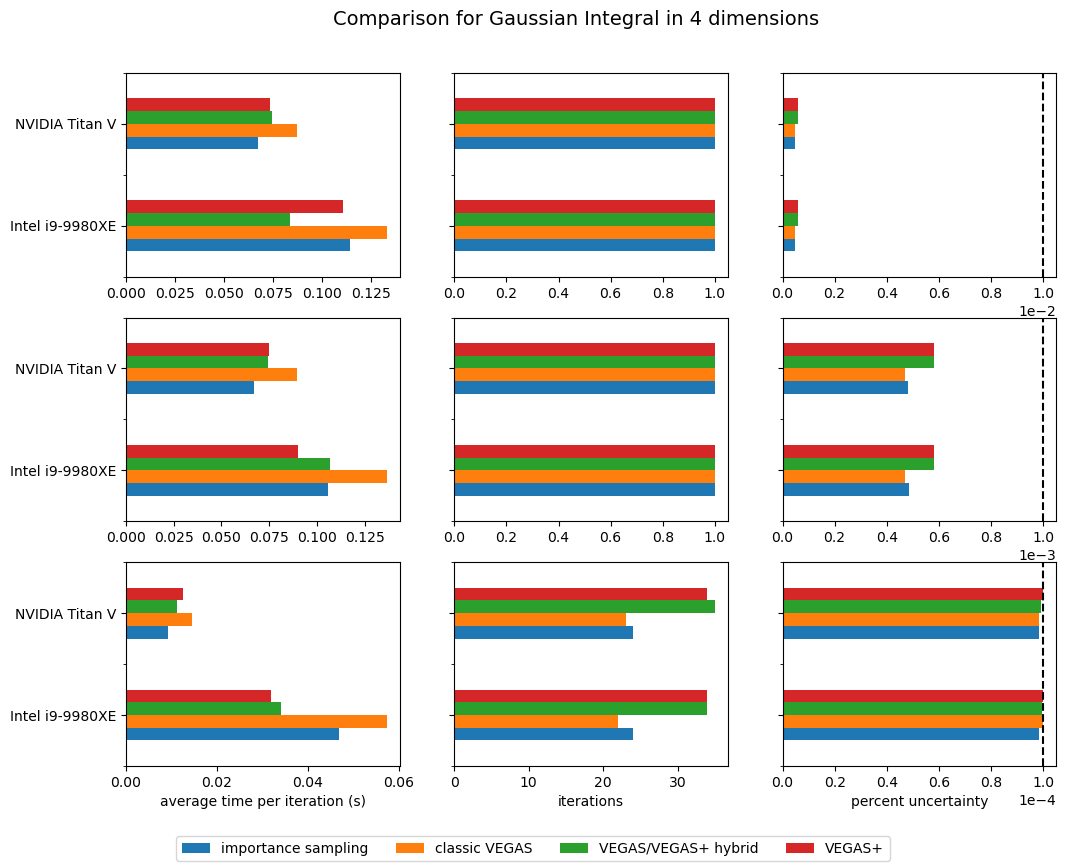
\includegraphics[ width = \columnwidth]{../tex/images/gauss4d_final.png}
		\end{figure}
	\end{column}
	\begin{column}{0.4 \textwidth}
		\vspace{1cm} 
		\begin{itemize}
			\item classic VEGAS is the most accurate integrator followed by the importance sampling
			\item the VEGAS+ integrators are not effective since we are dealing with an integrand with a non-diagonal sharp peak 
			\item benefits when running on GPU:  up to 3x improvement
		\end{itemize}
	\end{column}
	
\end{columns}
\begin{figure}
	\caption{Benchmark  for the Gaussian integral in 4 dimensions. From right to left are presented the average time per iteration (after the warm-up), the number of iterations needed to reach target accuracy and the percent uncertainty reached at the end of the simulation. From the first row to the last one the target accuracies (dashed in the last column) are at $10^{-2}$, $10^{-3}$ and $10^{-4}$ percent uncertainty.}
\end{figure}


\end{frame}

\begin{frame}{Gaussian Integral Benchmark - Dimension 8}
	\tiny
\vspace{-0.5cm}
\begin{columns}
	\begin{column}{0.6 \textwidth}
		\begin{figure}
			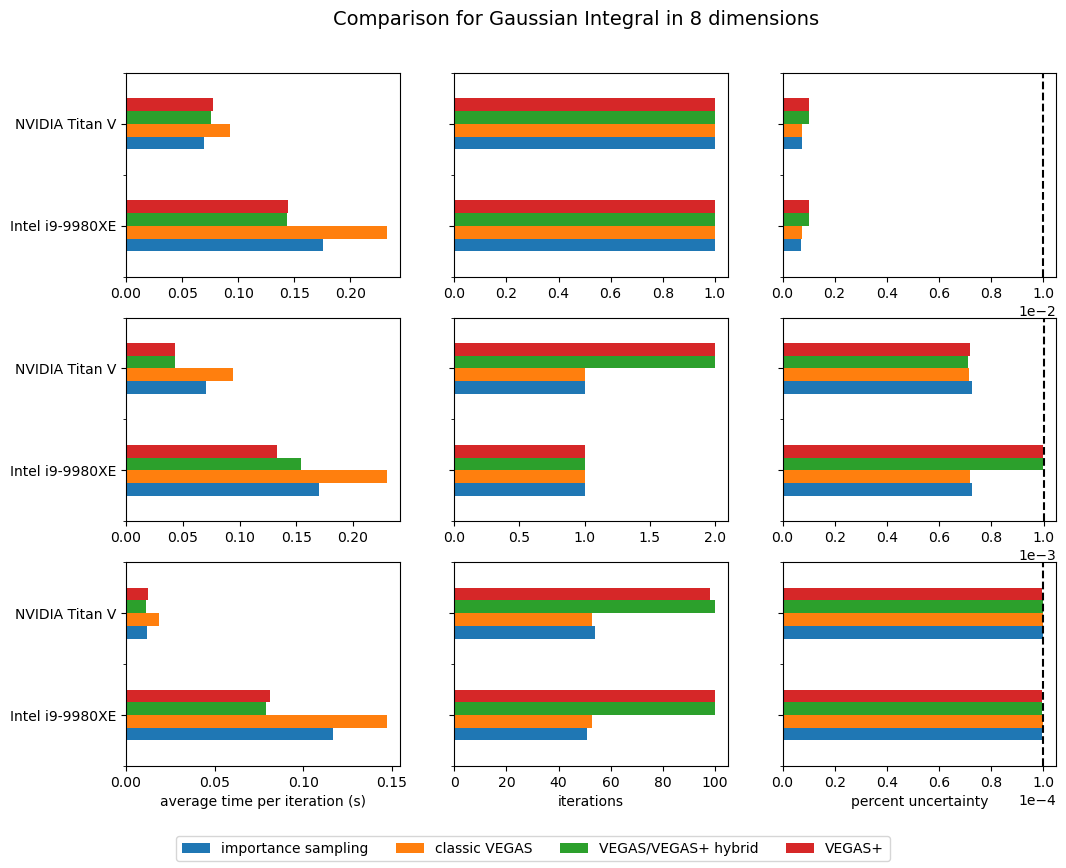
\includegraphics[ width = \columnwidth]{../tex/images/gauss8d_final.png}
		\end{figure}
	\end{column}
	\begin{column}{0.4 \textwidth}
		\vspace{1cm} 
		\begin{itemize}
			\item trend similar to the previous case with worst perfomance of VEGAS+ integrators
			\item VEGAS+ algorithm fastest when running on CPU
			\item significant improvements in the computational times thanks to the graph implementation and the larger number of iterations
		\end{itemize}
	\end{column}
	
\end{columns}
\begin{figure}
	\caption{Benchmark  for the Gaussian integral in 8 dimensions. From right to left are presented the average time per iteration (after the warm-up), the number of iterations needed to reach target accuracy and the percent uncertainty reached at the end of the simulation. From the first row to the last one the target accuracies (dashed in the last column) are at $10^{-2}$, $10^{-3}$ and $10^{-4}$ percent uncertainty.}
\end{figure}
\end{frame}

\begin{frame}{Gaussian Integral Benchmark - Dimension 12}
	\tiny
\vspace{-0.5cm}
\begin{columns}
	\begin{column}{0.6 \textwidth}
		\begin{figure}
			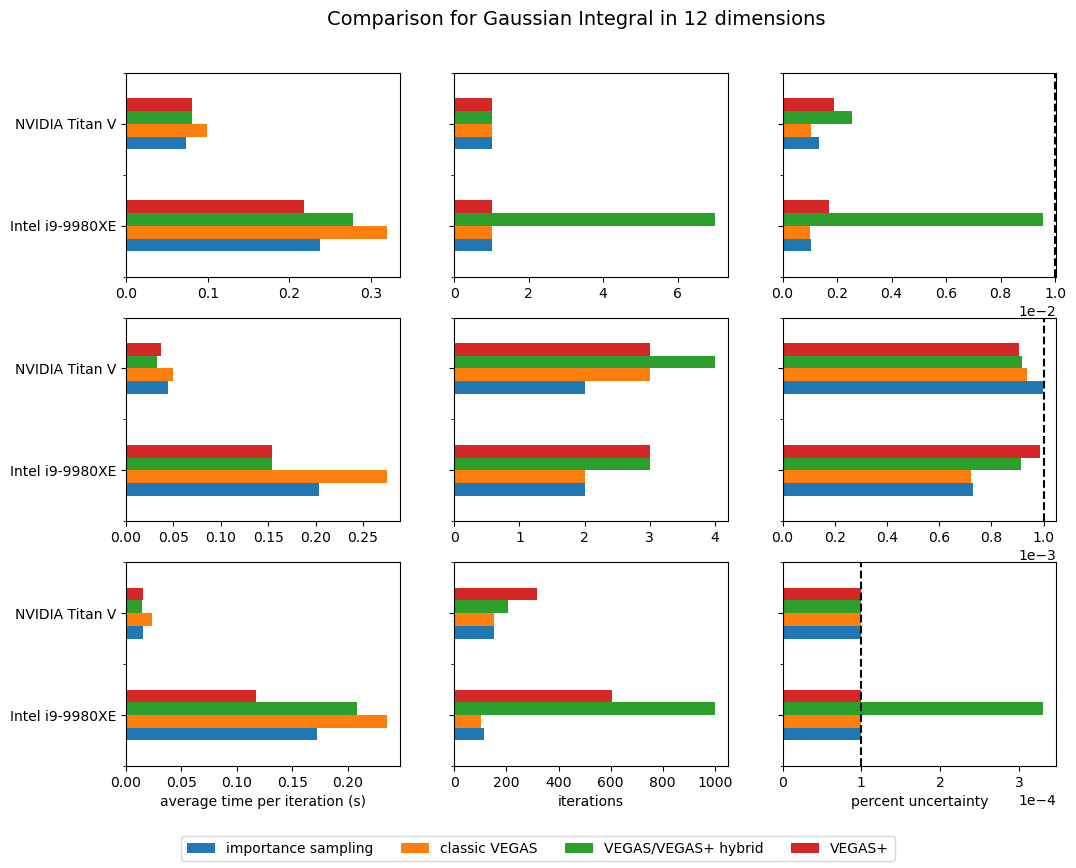
\includegraphics[ width = \columnwidth]{../tex/images/gauss12d_final.png}
		\end{figure}
	\end{column}
	\begin{column}{0.4 \textwidth}
		\vspace{1cm} 
		\begin{itemize}
			\item classic VEGAS and importance sampling reach the accuracy required using the same number of iterations
			\item worst performance of the VEGAS+ algorithm
			\item speed-up factors: importance sampling 11.5, classic VEGAS 10.1, VEGAS/VEGAS+ hybrid 14.8 and VEGAS+ 7.8.
		\end{itemize}
	\end{column}
	
\end{columns}
\begin{figure}
	\caption{Benchmark  for the Gaussian integral in 12 dimensions. From right to left are presented the average time per iteration (after the warm-up), the number of iterations needed to reach target accuracy and the percent uncertainty reached at the end of the simulation. From the first row to the last one the target accuracies (dashed in the last column) are at $10^{-2}$, $10^{-3}$ and $10^{-4}$ percent uncertainty.}
\end{figure}
\end{frame}


\begin{frame}{Drell-Yan at LO - partonic level}
	\vspace{-0.8cm}
%\begin{frame}
	\tiny
	\begin{columns}
		\begin{column}{0.6 \textwidth}
			\begin{figure}
				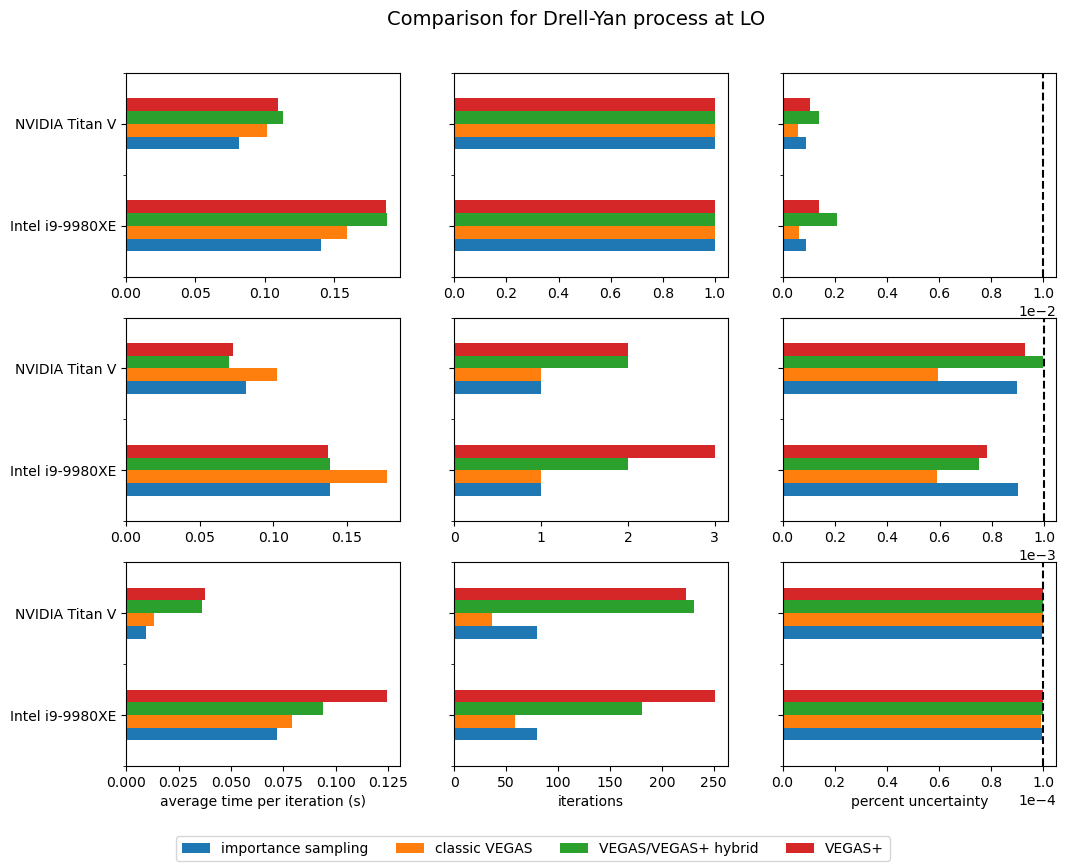
\includegraphics[ height = 6 cm]{../tex/images/pineappl_final.png}

			\end{figure}
		\end{column}
		\begin{column}{0.4 \textwidth}
			\vspace{1cm} 
			\begin{itemize}
				\item physical integral with dimension 3
				\item classic VEGAS is the best performing integrator
				\item importance sampling is the fastest integrator both on CPU and GPU
				\item the worst performance of VEGAS+ suggests a that the integral has a sharp peak easily found by the VEGAS grid
			\end{itemize}
		\end{column}
		
	\end{columns}
\begin{figure}
					
	\caption{Benchmark  for the partonic level cross section for the DY photon induced process  at LO. From right to left are presented the average time per iteration (after the warm-up), the number of iterations needed to reach target accuracy and the percent uncertainty reached at the end of the simulation. From the first row to the last one the target accuracies (dashed in the last column) are at $10^{-2}$, $10^{-3}$ and $10^{-4}$ percent uncertainty.}
\end{figure}
\end{frame}
%\begin{figure}
%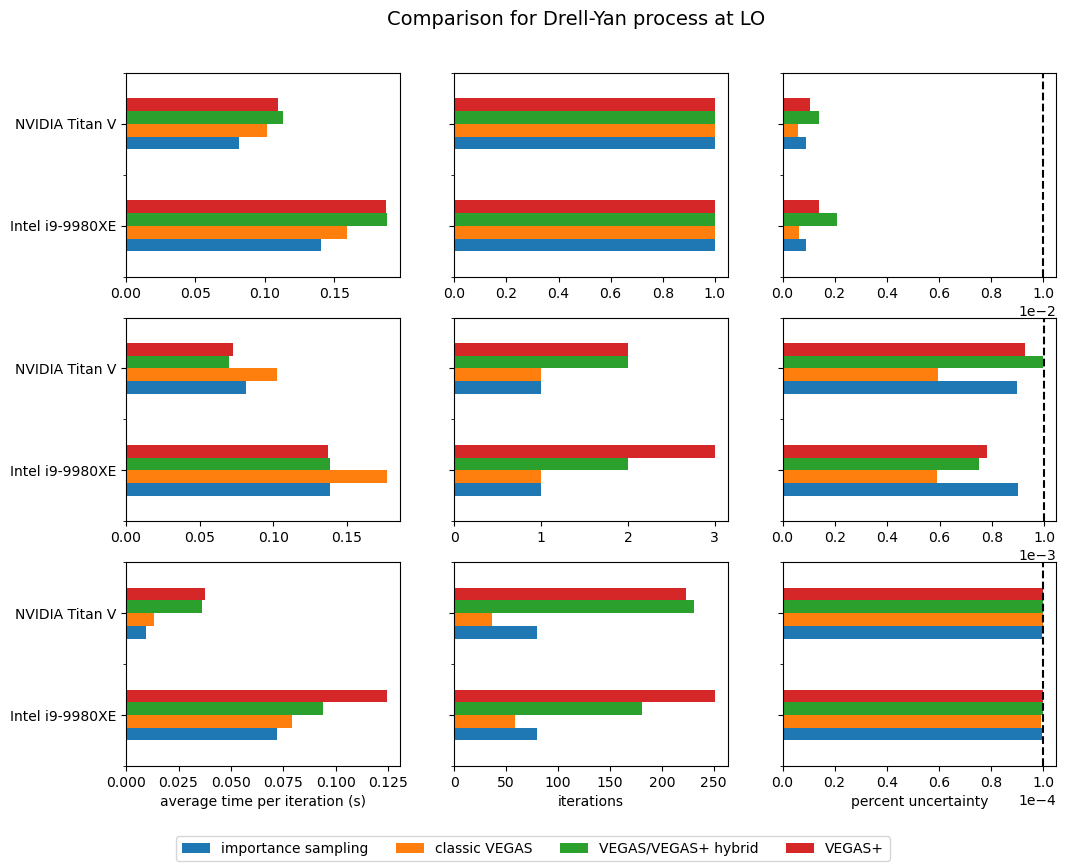
\includegraphics[height=0.7 \textheight]{../tex/images/pineappl_final.png}

%\end{figure}


%\end{frame}

\begin{frame}{Single Top Production at LO - partonic level}
	
		\vspace{-0.8cm}
	%\begin{frame}
	\tiny
	\begin{columns}
		\begin{column}{0.6 \textwidth}
			\begin{figure}
				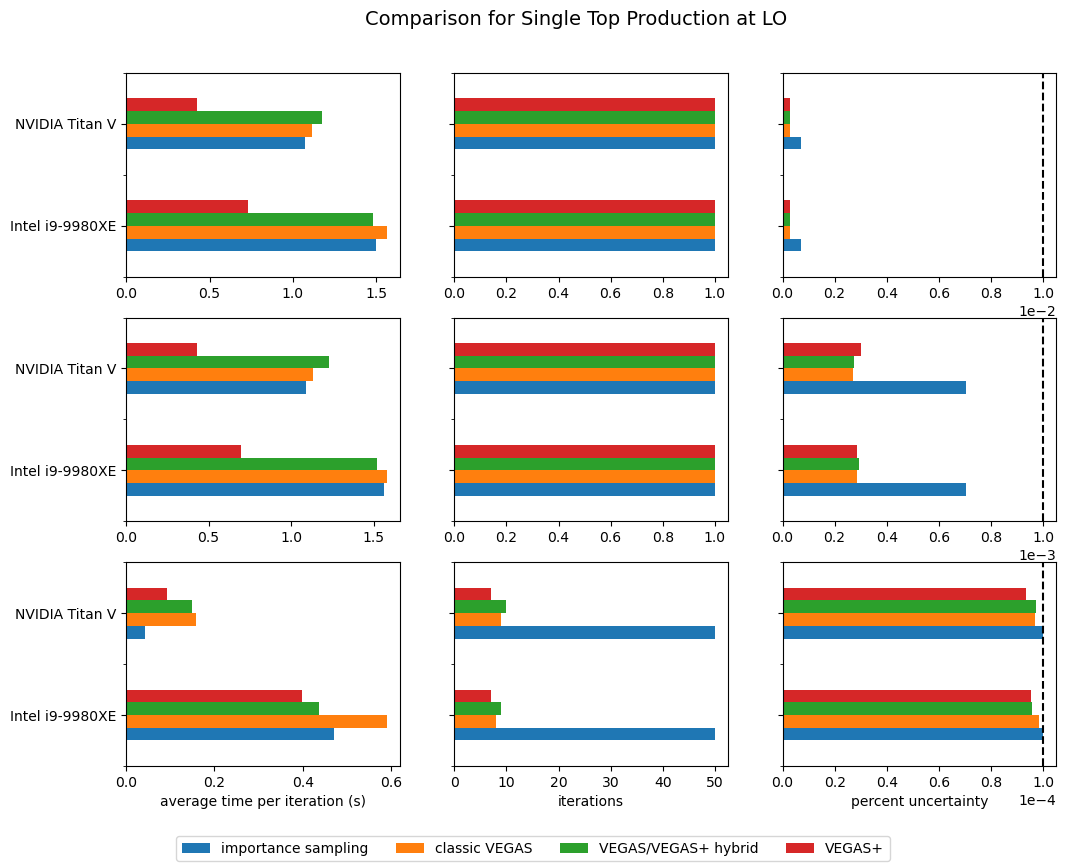
\includegraphics[ height = 6 cm]{../tex/images/singletop_final.png}
			\end{figure}
		\end{column}
		\begin{column}{0.4 \textwidth}
			\vspace{1cm} 
			\begin{itemize}
				\item physical integral of dimension 3
				\item the importance sampling is by far the less efficient integrator
				\item the adaptive stratified sampling of VEGAS+ is particulary effective for this integrand
				\item on GPU the importance sampling is still the fastest despite the worst performances
			\end{itemize}
		\end{column}
		
	\end{columns}
\begin{figure}
					\caption{Benchmark  for the partonic level cross section for the single $t$-quark production (t-channel)  at LO. From right to left are presented the average time per iteration (after the warm-up), the number of iterations needed to reach target accuracy and the percent uncertainty reached at the end of the simulation. From the first row to the last one the target accuracies (dashed in the last column) are at $10^{-2}$, $10^{-3}$ and $10^{-4}$ percent uncertainty.}
\end{figure}
	
	
	
\end{frame}
\begin{frame}{Vector Boson Fusion Higgs production at LO}
			\vspace{-0.8cm}
	%\begin{frame}
	\tiny
	\begin{columns}
		\begin{column}{0.6 \textwidth}
			\begin{figure}
				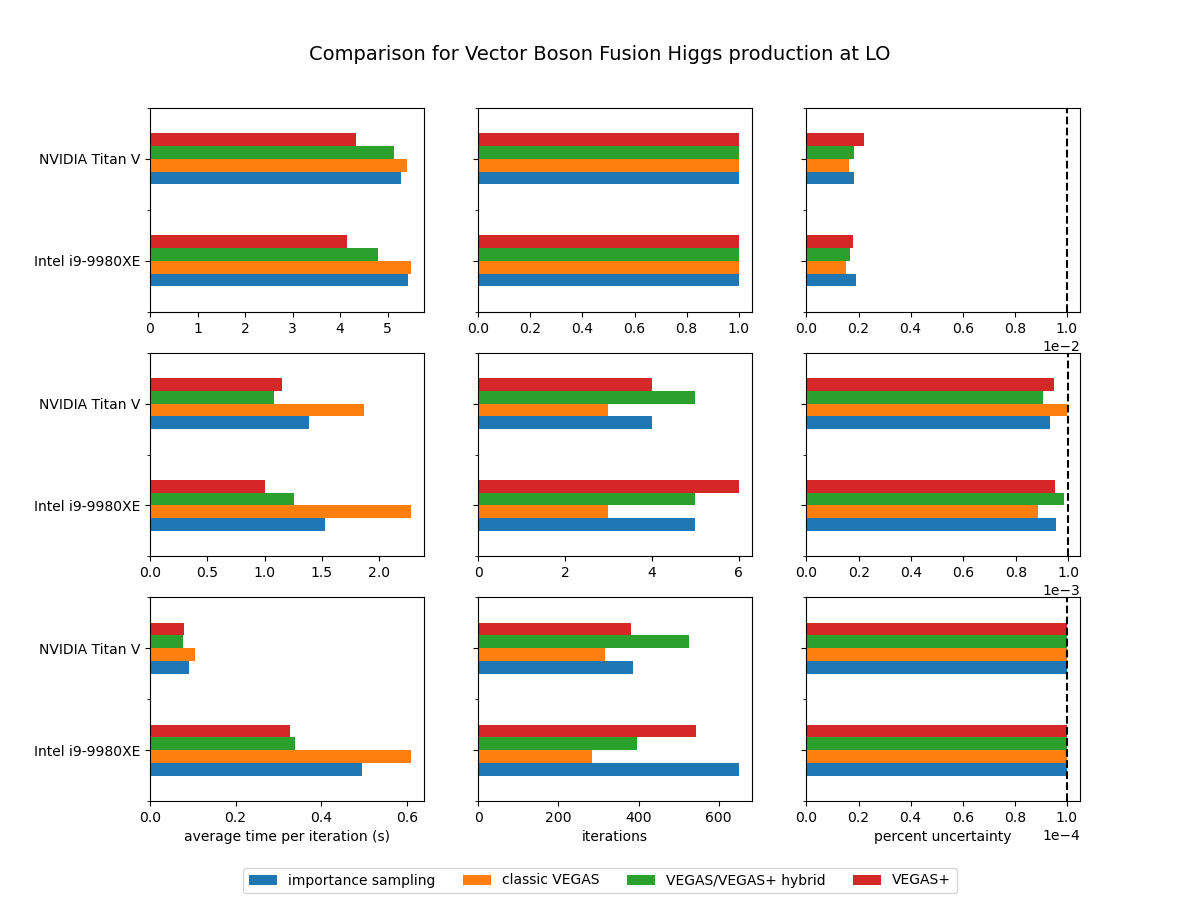
\includegraphics[ width = \columnwidth]{../tex/images/higgs_correct.png}
			\end{figure}
		\end{column}
		\begin{column}{0.4 \textwidth}
			\vspace{1cm} 
			\begin{itemize}
				\item physical integral of dimension 6 with convolution with PDFs
				\item classic VEGAS is the most efficient integrator overall
				\item significant benefits from GPU run, with speed-up factors between 4 and 6
				\item new algorithms more efficient than the importance sampling
			\end{itemize}
		\end{column}
		
	\end{columns}
\begin{figure}
					
	\caption{Benchmark  for the cross section for the vector boson fusion (VBF) Higgs production at LO. The set of PDFs is \texttt{NNPDF31\_nnlo\_as\_0118} From right to left are presented the average time per iteration (after the warm-up), the number of iterations needed to reach target accuracy and the percent uncertainty reached at the end of the simulation. From the first row to the last one the target accuracies (dashed in the last column) are at $10^{-2}$, $10^{-3}$ and $10^{-4}$ percent uncertainty.}
\end{figure}
	

	
	
\end{frame}


\begin{frame}{Average time per iteration CPU}
	\tiny
	\begin{columns}
		\begin{column}{0.7 \textwidth}
			\begin{figure}
									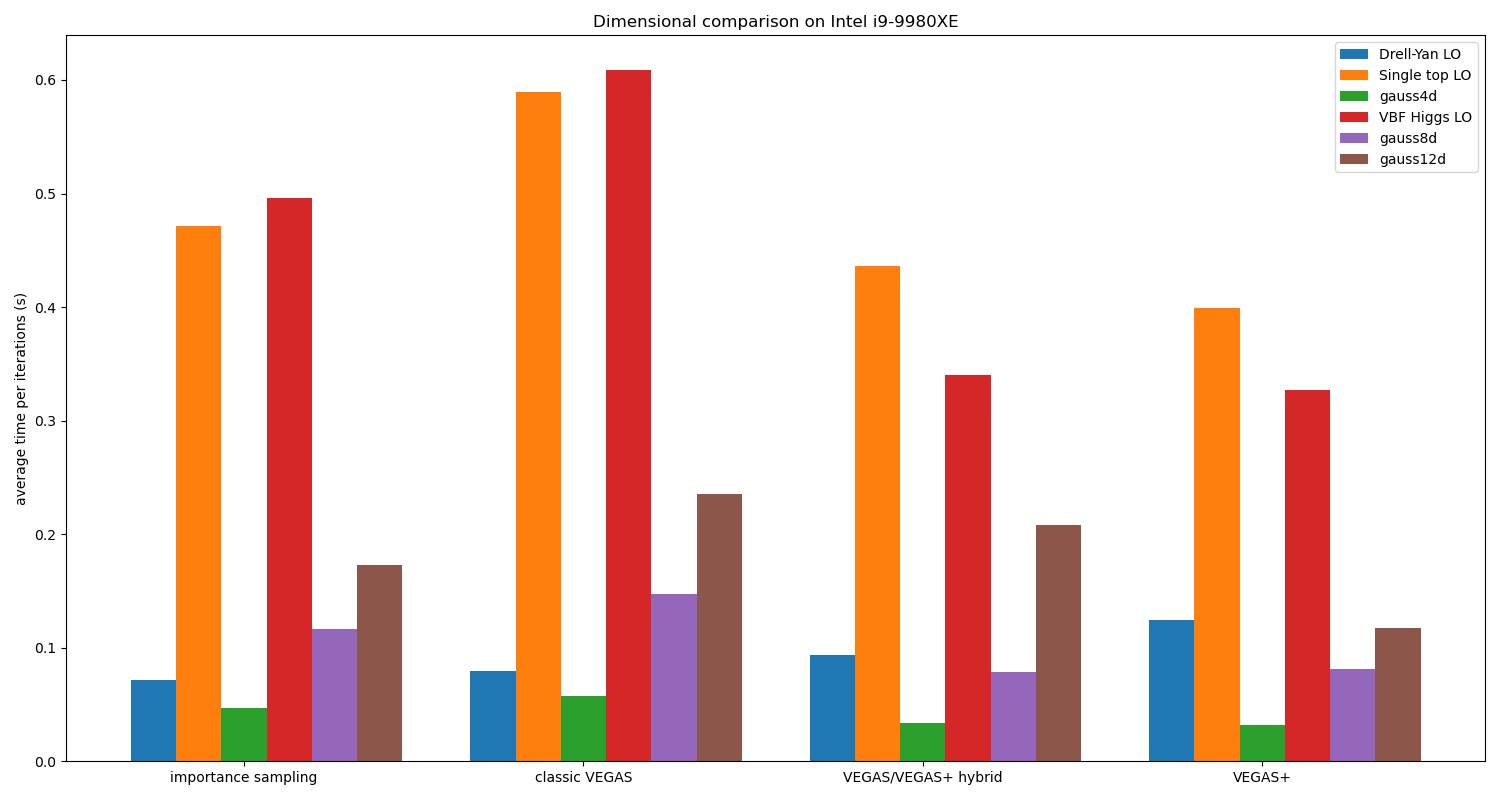
\includegraphics[width= \columnwidth]{../tex/images/CPU_final.png}
			\end{figure}

		\end{column}
	\hspace{-0.5cm}
	\begin{column}{0.3\textwidth}
					\vspace{0.7cm}
					
		\begin{itemize}

			\item VEGAS+ algorithms with shorter times when dealing with complex physical integrands such as Higgs or Top
		    \item VEGAS+ is the fastest when dealing with a 12-dim Gauss distribution
	\end{itemize}
	\end{column}
	\end{columns}
	\begin{figure}
		%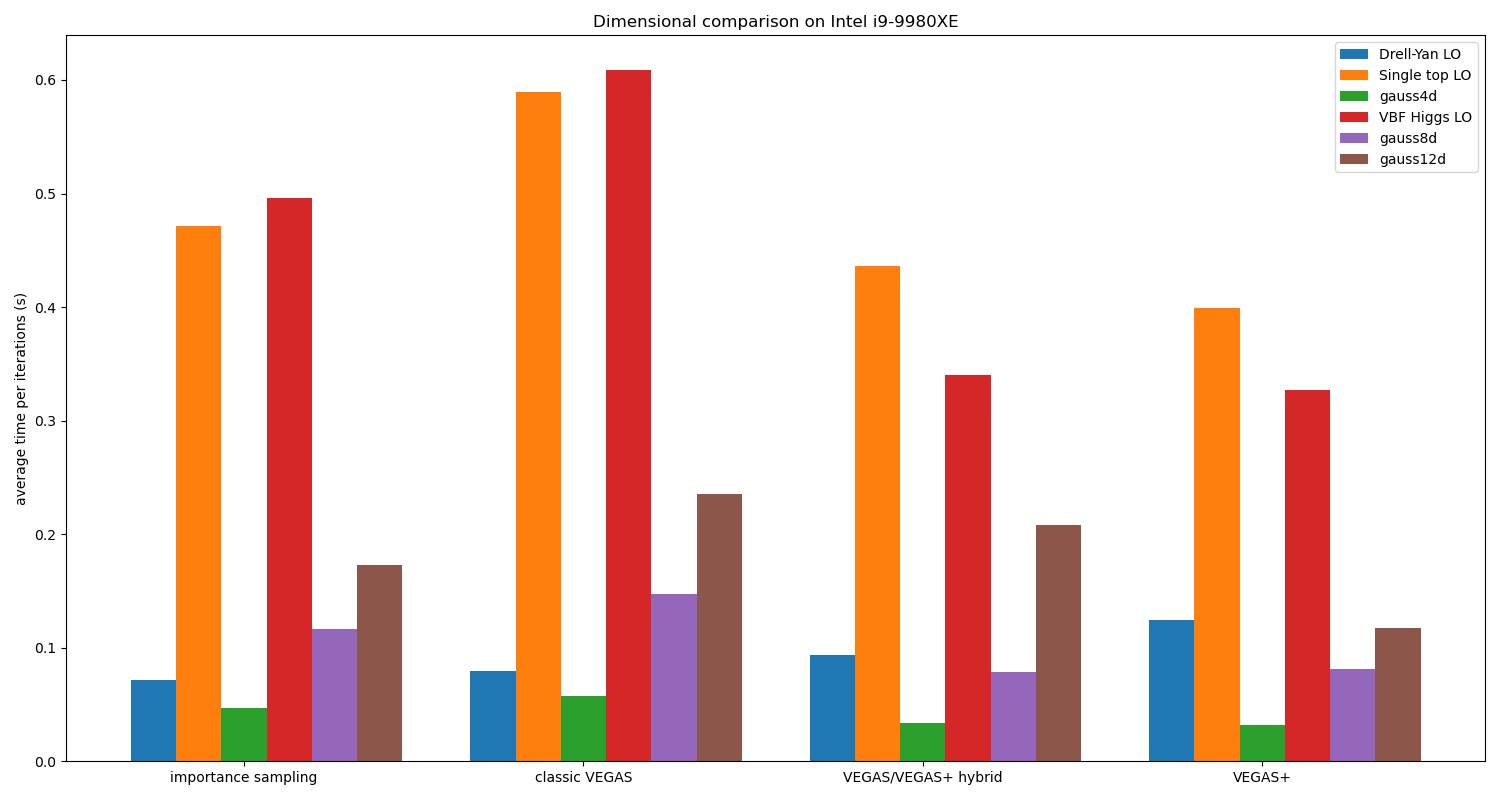
\includegraphics[height= 0.6 \textheight]{../tex/images/CPU_final.png}
		\caption{Average time per iteration (after the warm-up) for all the previously studied cases. The results are sorted by the integrand dimension for each integrator. All the integration are performed on the Intel i9-9980XE CPU. }
	\end{figure}

\end{frame}

\begin{frame}{Average time per iteration GPU}
	
		\tiny
	\begin{columns}
		\begin{column}{0.7 \textwidth}
			\begin{figure}
				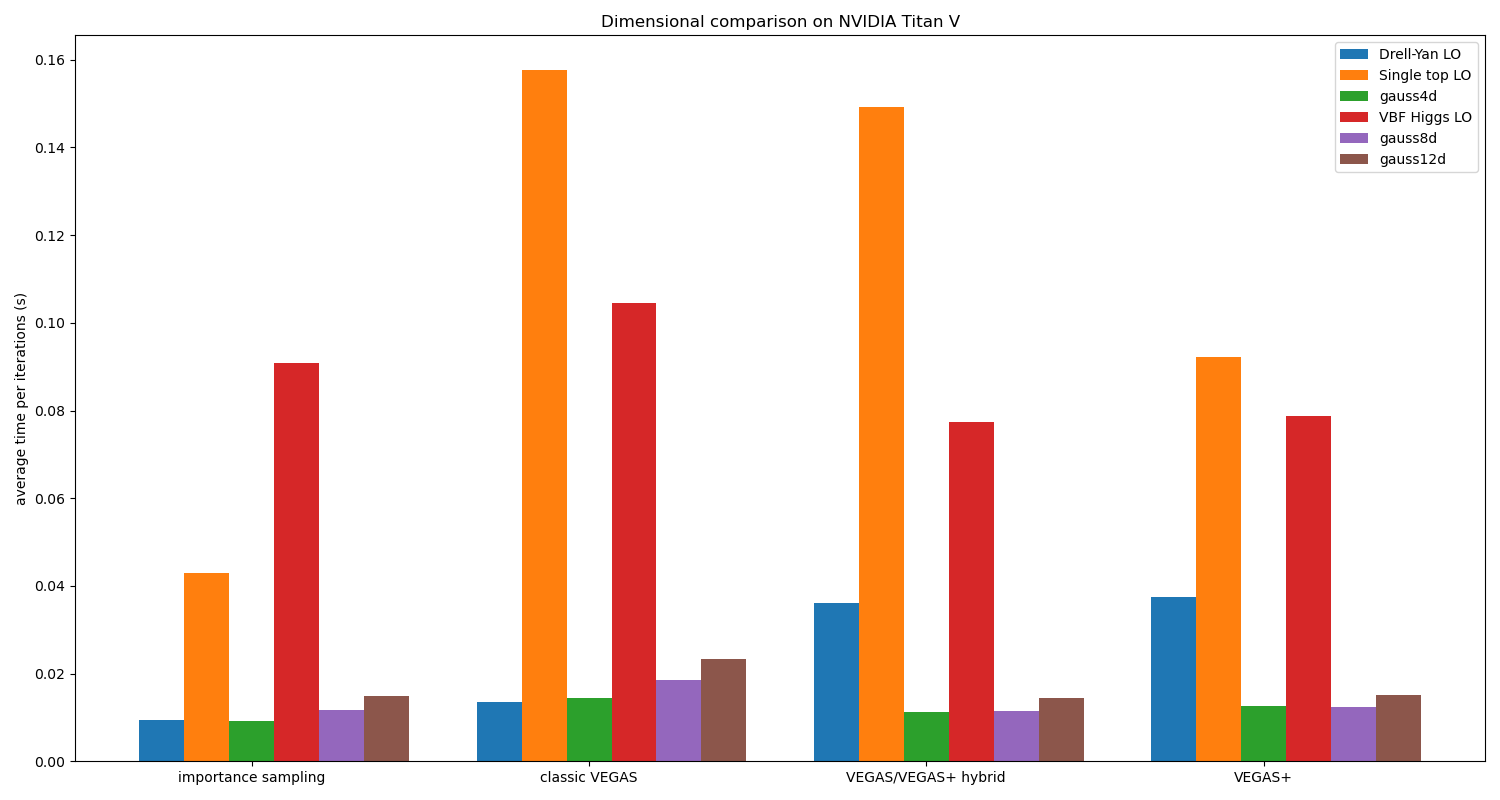
\includegraphics[width= \columnwidth]{../tex/images/GPU_final.png}
			\end{figure}
			
		\end{column}
			\hspace{-0.5cm}
		\begin{column}{0.3 \textwidth}
			\vspace{0.7cm}
			
			\begin{itemize}
				
				\item fastest integrator importance sampling
				\item for VBF Higgs the VEGAS+ algorithms are faster than the importance sampling
			\end{itemize}
		\end{column}
	\end{columns}
	\begin{figure}
		%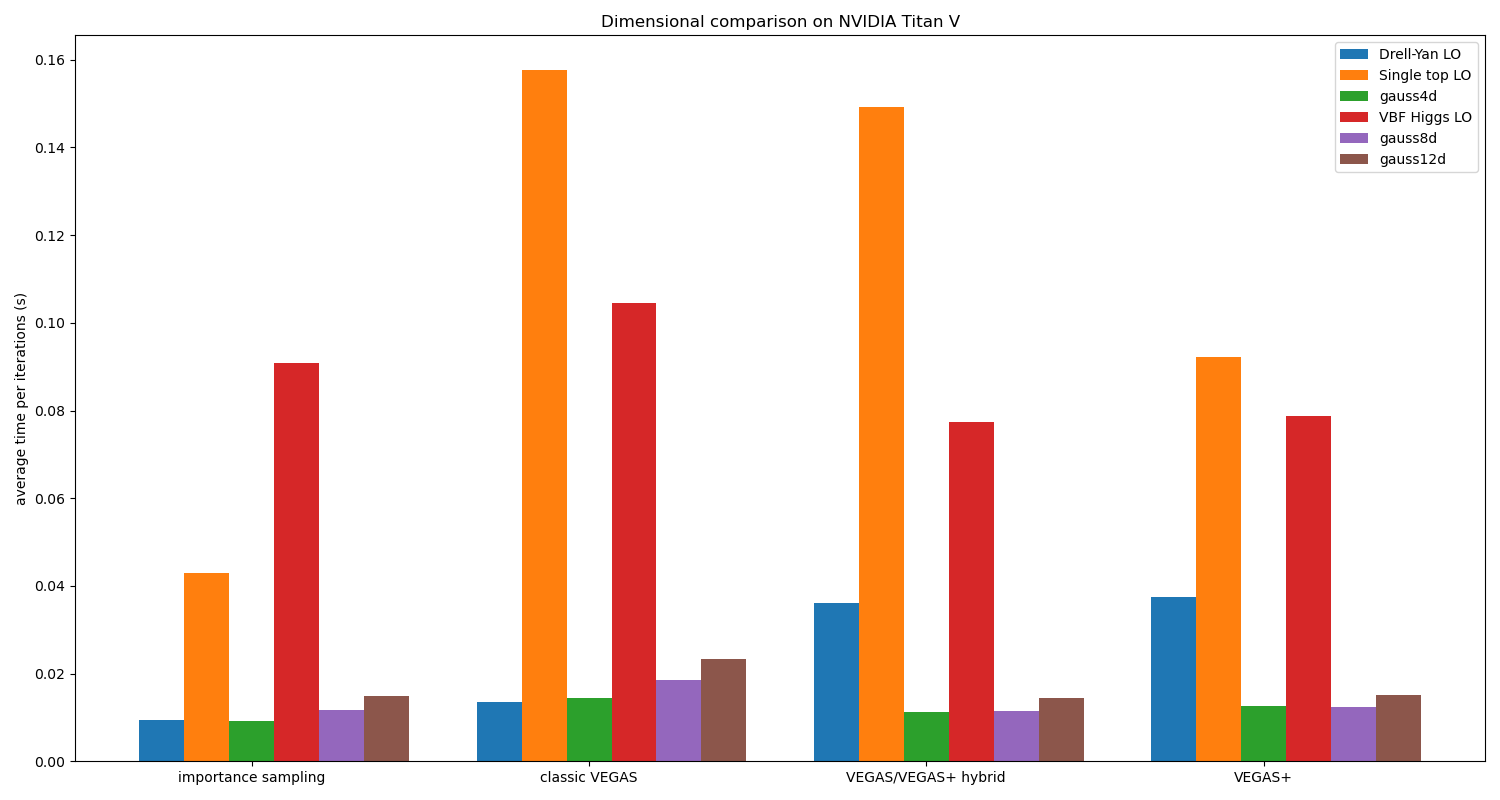
\includegraphics[height= 0.6 \textheight]{../tex/images/GPU_final.png}
		\caption{Average time per iteration (after the warm-up) for all the previously studied cases. The results are sorted by the integrand dimension for each integrator. All the integration are performed on the NVIDIA Titan V GPU. }
	\end{figure}

\end{frame}

	


\begin{frame}{Number of iterations}
	
		\tiny
	\begin{columns}
		\begin{column}{0.7 \textwidth}
			\begin{figure}
				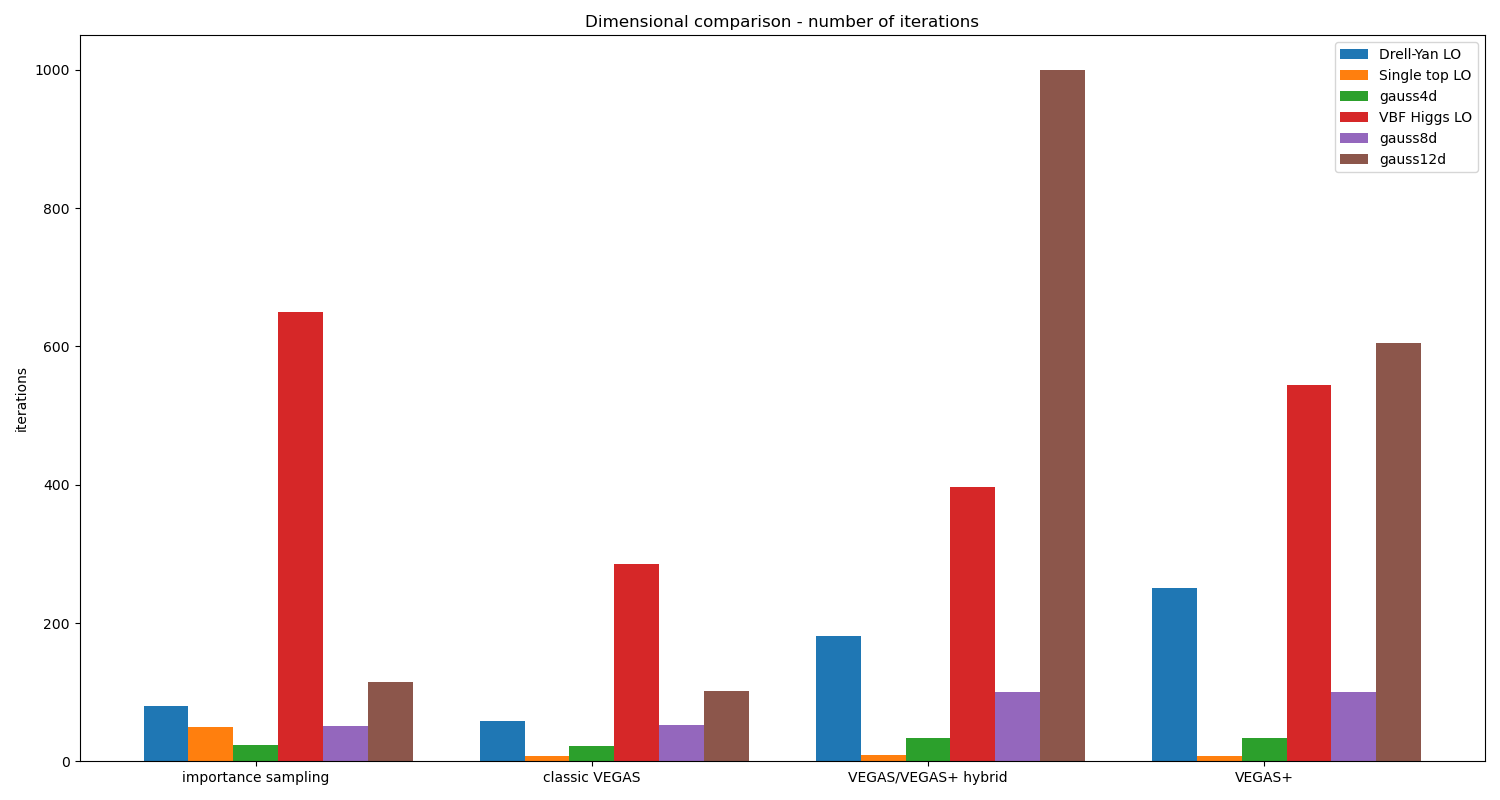
\includegraphics[width= \columnwidth]{../tex/images/iter_final.png}
			\end{figure}
			
		\end{column}
		\hspace{-0.5cm}
		\begin{column}{0.3 \textwidth}
			\vspace{1cm}
			
			\begin{itemize}
				
				\item classic VEGAS is the most efficient algorithm
				\item great performance of the new algorithms for the single Top production
				\item adaptive not effective with Gaussian due to the single sharp peak in high dimensions
			\end{itemize}
		\end{column}
	\end{columns}
	
		\begin{figure}
		%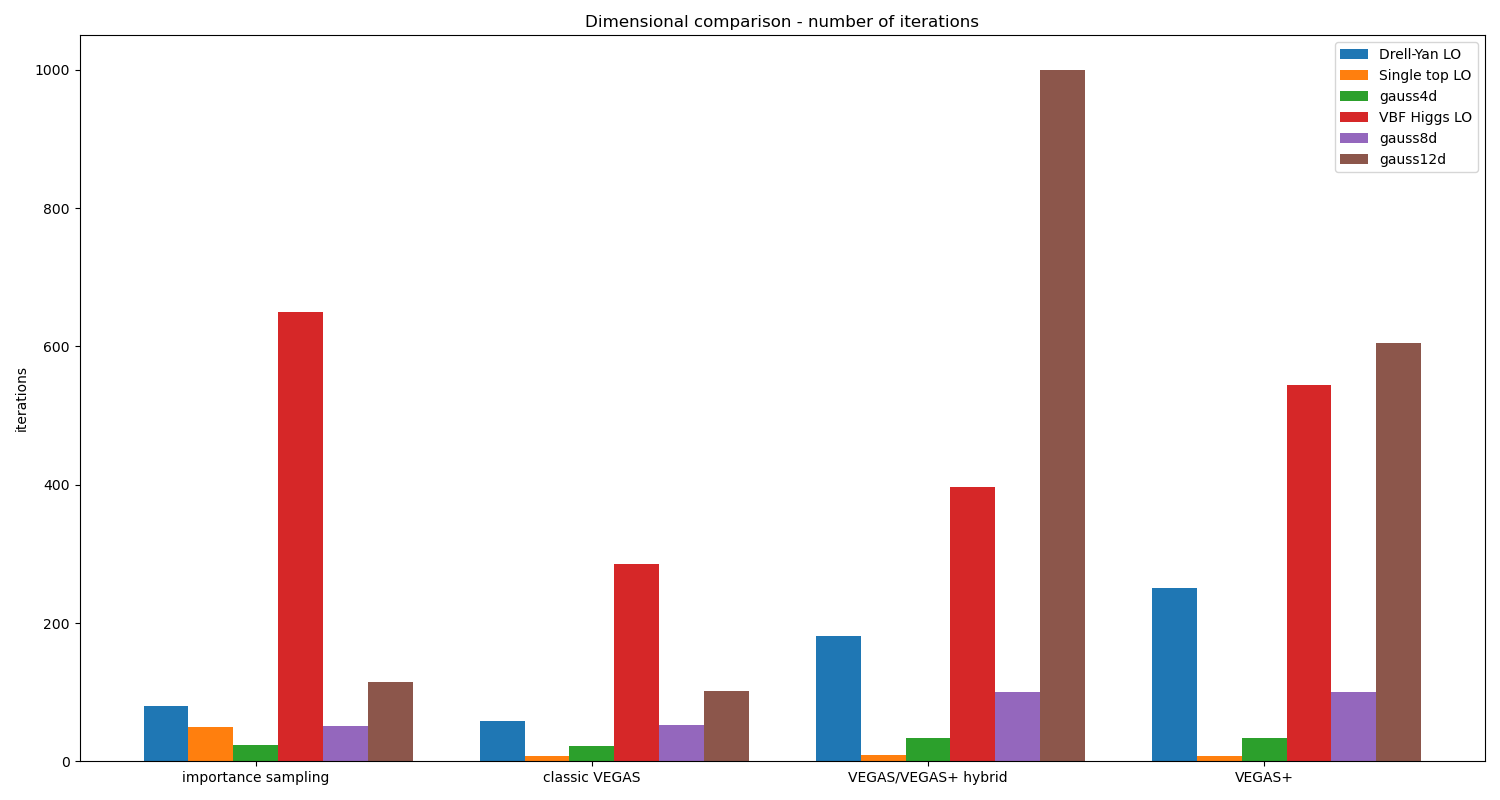
\includegraphics[height= 0.6 \textheight]{../tex/images/iter_final.png}
		\caption{Iterations needed to reach the accuracy of $10^{-4}$ percent uncertainty (after the warm-up) for all the previously studied cases. The results are sorted by the integrand dimension for each integrator. All the integration are performed on the Intel i9-9980XE CPU. }
	\end{figure}
	
\end{frame}


\begin{frame}{Conclusions}
	\scriptsize
	In this thesis we have considered the problem of evaluating high-dimensional integrals in the context of HEP and 
	the relative computational costs.
	
	We focus on implementing the \texttt{VEGAS+} algorithm and we empower it by taking advantage of hardware acceleration.
	
	The results of the benchmark show  that:
	
	\begin{itemize}
		\item the implementation benefits from highly parallel scenarios $\Rightarrow$ speed-up factors up to 10
		\item on CPU VEGAS+ is the fastest integrator
		\item new integrators more accurate when dealing with HEP integrands (Higgs or Single Top)
		\item classic VEGAS, a variation of VEGAS+, is the most efficient integrator
		
	\end{itemize}
\vspace{1cm}

\textbf{Future developments:}
\begin{itemize}
	\item implement new MC integration algorithms in \texttt{VegasFlow}
	\item machine-learning techniques for importance sampling
\end{itemize}
	
\end{frame}

\section{Back-up slides}
\begin{frame}{Reducing the variance}
	\tiny
	\begin{columns}
		\begin{column}{0.5 \textwidth}
			\textbf{Importance sampling}
			\begin{align*}
				I & = \underbrace{\int_{V}   f(\textbf{x})  d \textbf{x}}_{\substack{\text{integral of } f  \text{ with} \\ \text{uniform sampling}}}  =\int_{V}   \frac{f(\textbf{x})}{ p(\textbf{x})} p(\textbf{x})  d\textbf{x} \\
				& =\underbrace{\int_{V}  \frac{f(\textbf{x})}{ p(\textbf{x})} dP(\textbf{x}) }_{\substack{\text{integral of } f/p \\ \text{with sampling } dP}} 
			\end{align*}
			
			
			Therefore, we can estimate the integral as
			\begin{equation*}
				I_\text{MC}= V \langle f/p \rangle_P 
			\end{equation*}
			\begin{equation*}
				\sigma^2_I \approx \sigma^2_\text{MC} = \frac{V^2}{N-1} \underbrace{\bigg[\langle (f/p)^2 \rangle_P - \langle f/p \rangle^2_P \bigg] }_{\substack{= 0 \text{ for } f = p}}
			\end{equation*}
			
			\textbf{Aim}: find a function $p$ that resemble the shape of $f$ through adaptive recursive techniques.
			
			\vspace{0.05cm}
			
			\textbf{Disadvantage}:
		\end{column}
		\begin{column}{0.5 \textwidth}
			\textbf{Stratified Sampling}
			
			\vspace{0.3cm}
			If we divide the integration volume in two subvolumes $a$ and $b$, another estimator for the mean value of the function f is 
			\begin{equation*}
				\langle f  \rangle ' \equiv \frac{1}{2} (  \langle f \rangle_a + \langle f \rangle_b ) 
			\end{equation*}
			with variance
			\begin{equation*}
				\text{Var}(\langle f \rangle ') = \dfrac{1}{2N} \big[ \text{Var}_a(f) + \text{Var}_b(f)\big] 
			\end{equation*}
			
			While the variance of $f$ is 
			\begin{equation*}
				\text{Var}(f) = \underbrace{\frac{1}{2} [ \text{Var}_a(f) + \text{Var}_b(f)]}_{\propto \text{Var}(\langle f \rangle ') } + \underbrace{\frac{1}{4} ( 
					\llangle f \rrangle_a - \llangle f \rrangle_b)^2}_{ \geq 0} \ .
			\end{equation*}
			\vspace{0.05cm}
			
			\textbf{Aim}: divide the integration domain in several subvolumes to reduce the variance
			\vspace{0.05cm}
			
			\textbf{Disadvantage}: we need at leat two points in each subvolume to compute the variance.
		\end{column}
	\end{columns}
\end{frame}

\begin{frame}{Theoretical prediction and Standard Model}
	\scriptsize
	In a generic Quantum Field Theory we can predict the value of an observable, such as the differential cross section, in the following way
	\begin{equation}
		\label{sigma}
		d \sigma = \frac{1}{4 E_A E_B |v_A - v_B|} \  \underbrace{~ d\Pi_n ~}_{\substack{\text{phase-space}\\ \text{density}}} ~ \times   
		\underbrace{|\mathcal{M}(k_A, k_B \to p_1, ..., p_n)|^2}_{\text{invariant scattering amplitude}}  
	\end{equation}
	The integration over the phase-space is of the form 
	\begin{equation}
		\int d\Pi_n  = \bigg( \prod_{i=1}^{n}\int
		\frac{d^3 p_i}{(2 \pi)^3}
		\frac{1}{2 E_i} \bigg) (2\pi)^4 \delta^{(4)}\big(k_A+ k_B- \sum_{i=1}^n p_i\big) \ ,
	\end{equation} 
	which corresponds to a $3n-4$ dimensional integral.
	
	The matrix element is computed using Feynman diagrams by combining the real emissions and the loop corrections to avoid IR and UV divergences.
	
	
	
	
	\begin{equation}
		\mathcal{M} = 
		\begin{cases}
			\mathcal{M}^{\text{tree}}  + \mathcal{M}^{\text{1-loop}} + \mathcal{M}^{\text{2-loops}} + \dots \  \quad &\text{quantum corrections} \\
			\mathcal{M}^{\text{tree}}  + \mathcal{M}^{\text{1-leg}} + \mathcal{M}^{\text{2-legs}} + \dots  \quad &\text{real emissions}
		\end{cases}
	\end{equation}
	
	The final expression will be of the form
	\begin{equation}
		d\sigma = d\sigma^{\text{LO}} + d\sigma^{\text{NLO}} + d\sigma^{\text{NNLO}} \dots  \ .
	\end{equation}
	
	%which leads to an expression of the form
	%\begin{equation}
	%	d\sigma = d\sigma^{\text{LO}} + d\sigma^{\text{NLO}} + d\sigma^{\text{NNLO}} \dots  \ .
	%\end{equation}
\end{frame}

\begin{frame}{}
	\scriptsize
	By aiming at higher precisions we will encounter several complex multi-dimensional integrals:
	\begin{itemize}
		\item adding loop to a diagram $\Rightarrow$ $D_\text{loop} = D_\text{diagram} + 4$
		\item adding external leg to a diagram $\Rightarrow$ $D_\text{leg} = D_\text{diagram} + 3$
		\item more complex diagrams $\Rightarrow$ more difficult integral evaluation
		\item in QCD we also need to compute the convolution with the Parton Density Functions (PDFs) according to the QCD factorization theorem
		\begin{equation}
			\label{QCD fact}
			d\sigma = \sum_{a,b}\int_0^1 dx_a dx_b \sum_F \int d\Phi_F \underbrace{f_{a/h_1}(x_a,\mu_F) f_{b/h_2}(x_b,\mu_F) }_\text{parton density functions} \underbrace{d\hat{\sigma}_{ab \rightarrow F}}_{\substack{\text{partonic}\\ \text{cross} \\ \text{section}}} \ .
		\end{equation}
	\end{itemize}
	The squared matrix element $|\mathcal{M}^2|$ is difficult to sample since it is particularly peaked in a small region of the integration domain, usually near kinematics divergences. 
	
	These regions become even smaller for high-dimensional integrals:
	\begin{equation}
		\frac{V_{\text{hypersphere}}}{V_{\text{hypercube} }} = \frac{1}{2^D} \frac{\pi^{\frac{D}{2}}}{\Gamma\big(\frac{D}{2} + 1\big)} \approx  \bigg( \frac{\sqrt{\pi}}{2} \bigg)^D \xrightarrow{D \rightarrow  \infty} 0 \ ,
	\end{equation}
	
\end{frame}

\begin{frame}{\texttt{VEGAS}}
	\tiny
	\texttt{VEGAS} is an algorithm for adaptive multi-dimensional MC integration implemented by Lepage in 1977.
	It is the main drive for QCD fixed-order calculations programs such as \texttt{MCFM}, \texttt{NNLOJET}, \texttt{MG5} and \texttt{Sherpa}.
	\vspace{0.3cm}
	
	\textbf{Importance Sampling}
	
	The sampling distribution used is \emph{separable}
	\tiny
	\begin{equation*}
		p \propto g(x_1,x_2,x_3,\dots,x_n) = g_1(x_1)g_2(x_2)g_3(x_3)\dots g_n(x_n) \ .
	\end{equation*}
	
	\begin{columns}
		\begin{column}{0.5 \textwidth}
			The algorithm divides the integration domain in subintervals with probability
			\begin{equation*}
				g_i(x) = \frac{1}{N \Delta x_i} 
			\end{equation*}
			
			after each iteration the intervals $\Delta x_i$ are adjusted iteratively using the quantity
			
			\begin{equation*}
				\tiny{d_i \equiv \frac{1}{n_i} \sum_{x_j \in \interval{x_i - \Delta x_i}{x_i} } f^2(\textbf{x}) \approx \Delta x_i \int_{x_i - \Delta x_i}^{x_i} d\textbf{x} f^2(\textbf{x})  }
			\end{equation*}
			
			
		\end{column}
		\begin{column}{0.5 \textwidth}
			\begin{equation*}
				\int_0^1 d^4 x \big(e^{-100(\textbf{x}- \textbf{r}_1)^2} + e^{-100(\textbf{x}- \textbf{r}_2)^2} \big) 
			\end{equation*}
			\vspace{-0.5cm}
			\begin{figure}[h]
				\centering
				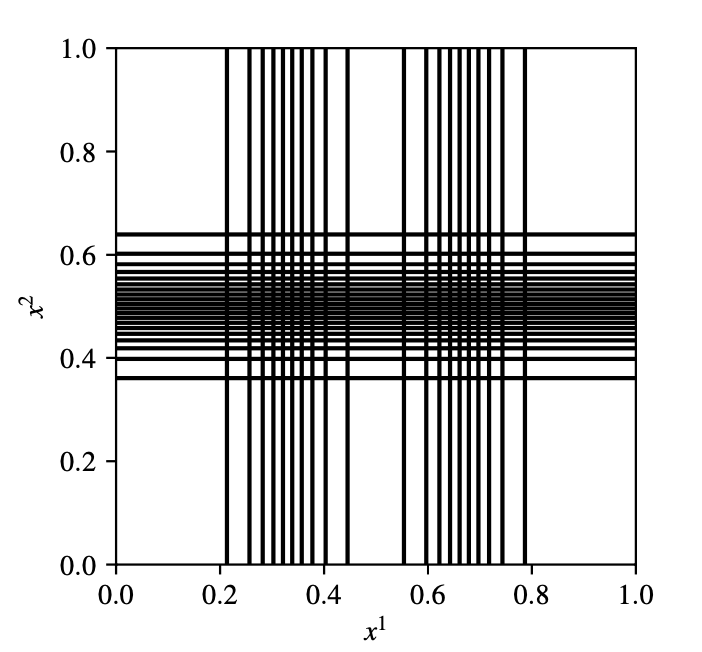
\includegraphics[height = 4cm]{../tex/images/vegas_grid.png}
				%\label{CPU cost}
			\end{figure}
			\begin{equation*}
				\textbf{r}_1 = (0.33, 0.5, 0.5, 0.5) 
			\end{equation*}
			\begin{equation*}
				\textbf{r}_2 = (0.67, 0.5, 0.5, 0.5)
			\end{equation*}
		\end{column}
	\end{columns}
\end{frame}

\begin{frame}
	\scriptsize
	\textbf{Stratified sampling}
	\begin{itemize}
		\item Each axis is divided into a fixed number of stratifications
		$N_\text{st} = \lfloor (N_\text{ev}/2)^{1/D}\rfloor $
		resulting in $N_\text{st}$ hypercubes.
		\item Every hypercube is sampled with $n_\text{ev}$ points : 	$n_\text{ev} = \lfloor (N_\text{ev}/N_\text{st}^D)\rfloor \ge 2$
		\item The integral and the variance are computed as
		\begin{equation*}
			\hspace{-2cm} I = \frac{V}{N_\text{st}^D}\sum_h \bigg(\frac{1}{n_\text{ev}} \sum_{\textbf{x} \in h} f(\textbf{x}) \bigg) = \sum_h I_h \quad , \quad \sigma^2_I = \sum_h \sigma^2_h 
		\end{equation*}
	\end{itemize}
	\vspace{0.5cm}
	\textbf{Limitations of \texttt{VEGAS}}
	\begin{itemize}
		\item not all integrands are separable
		\item stratified sampling uneffective for high-dimensional integrals
	\end{itemize}
\end{frame}

\begin{frame}{\texttt{VEGAS+} algorithm}
	\scriptsize
	\textbf{Problem}: \texttt{VEGAS} (importance + stratified sampling) struggles with non-separable integrals. 
	
	\textbf{Solution}: \texttt{VEGAS+} (importance + \emph{adaptive} stratified sampling).
	
	\vspace{0.3cm}
	
	\textbf{Adaptive stratified sampling}
	
	Each hypercube $h$ is sampled with a different number of points $n_h \neq n_\text{ev}$ which are adjusted iteratively. The integral and the variance are now computed as
	$$ I = \frac{V}{N_\text{st}^D}\sum_h \frac{1}{n_h} \sum_{\textbf{x} \in h} f(\textbf{x})  = \sum_h I_h  \quad , \quad \sigma^2_I = \sum_h  \frac{\sigma^2_h}{n_h} $$
	
	\texttt{VEGAS+} algorithm:
	\begin{enumerate}
		\item Choose number of stratifications $N_\text{st} = \lfloor (N_\text{ev}/4)^{1/D}\rfloor $
		\item Accumulate the variance in each hypercube:
		$$ \sigma^2_h \approx \frac{V_h^2}{n_h} \sum_{\textbf{x} \in V_h} f^2(\textbf{x}) - \bigg( \frac{V_h}{n_h} \sum_{\textbf{x} \in V_h} f(\textbf{x})\bigg)^2  $$
		\item Replace the variance with $d_h$ : $d_h \equiv \sigma_h^\beta$ with $\beta \geq 0$
		\item Recalculate the number of samples for each hypercube for the next iteration
		$$ n_h = \text{max} \big(2, d_h / \sum_{h'} d_{h'}\big)  $$
	\end{enumerate}
	
\end{frame}

\begin{frame}{A new implementation \texttt{VegasFlowPlus}}
	\scriptsize
	Novel implementation of the \texttt{VEGAS+} algorithm within \texttt{VegasFlow}: \texttt{VegasFlowPlus}.	 
	\begin{columns}
		\begin{column}{0.6 \textwidth}
			\begin{figure}
				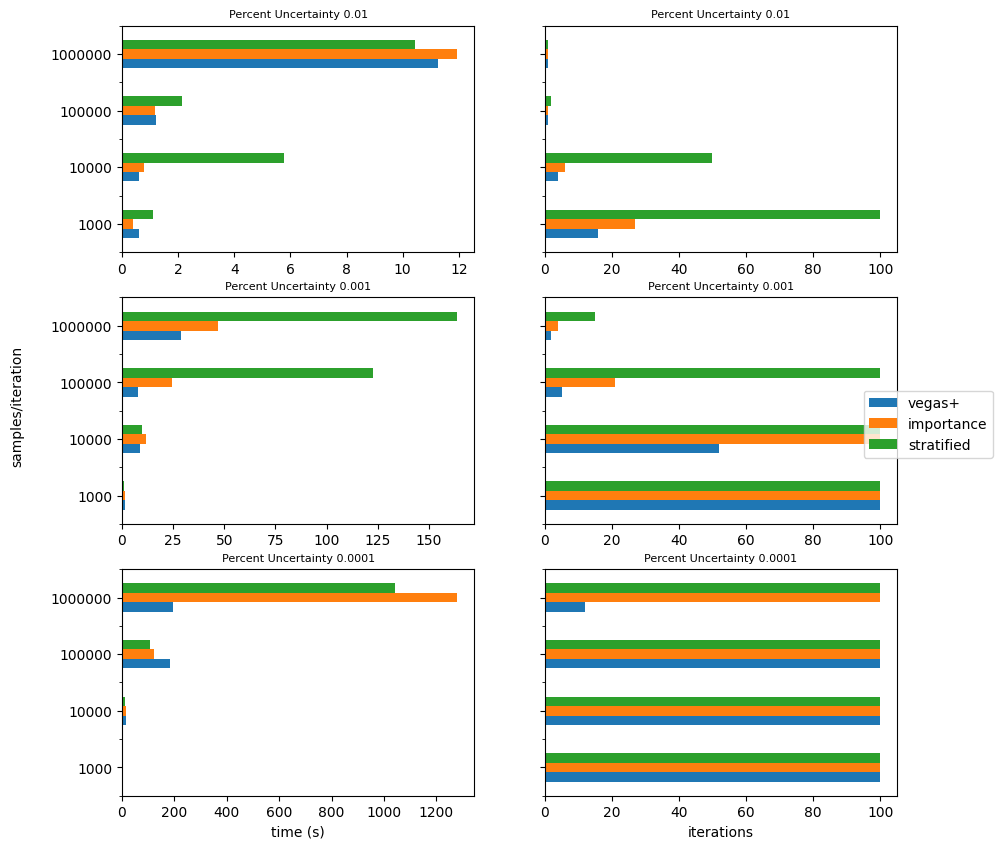
\includegraphics[ height = 6cm]{../tex/images/dy_aa.png}
			\end{figure}
		\end{column}
		\begin{column}{0.4 \textwidth}
			\tiny
			\vspace{0.7cm}
			
			\textbf{Motivation}: Several tests showed that \texttt{VEGAS+} 	can outperform the importance sampling of \texttt{VEGAS}, especially for physical integrands.
			
			\vspace{1cm}
			
			For the DY LO partonic level cross setion \texttt{VEGAS+} converge within the limit of 100 iterations when aiming at 0.0001\%  percent uncertainty.
			
			\vspace{1cm}
			
			These tests were performed with the single CPU implementation of \texttt{VEGAS} and \texttt{VEGAS+} currently available at \url{https://github.com/gplepage/vegas}
			
		\end{column}
		
	\end{columns}
\end{frame}

\begin{frame}{Implementation of \texttt{VegasFlowPlus}}
	\scriptsize
	\textbf{Details of the implementation}
	\begin{itemize}
		\item Class derived from the \texttt{VegasFlow} integrator (same importance sampling algorithm)
		\item Adding stratified sampling : \texttt{generate\_samples\_in\_hypercubes} + other modifications
		\item New feature of \texttt{VEGAS+}: \texttt{redistribute\_samples}
	\end{itemize}
	
	\vspace{2cm}
	
	\textbf{Problems during the implementation}:
	\begin{itemize}
		\item Number of events not constant $\Rightarrow$ require \texttt{input\_signature}
		\item Memory problem caused by \texttt{tf.repeat} $\Rightarrow$ limit on number of hypercubes
	\end{itemize}
\end{frame}

	
	
\end{document}